\documentclass[10pt]{article}
\usepackage[utf8]{inputenc}
\usepackage[T1]{fontenc}
\usepackage{amsmath}
\usepackage{amsfonts}
\usepackage{amssymb}
\usepackage[version=4]{mhchem}
\usepackage{stmaryrd}
\usepackage{graphicx}
\usepackage[export]{adjustbox}
\graphicspath{ {./images/} }
\usepackage{hyperref}
\hypersetup{colorlinks=true, linkcolor=blue, filecolor=magenta, urlcolor=cyan,}
\urlstyle{same}
\usepackage{bbold}

\title{Self-supervised Learning }


\author{Dec 12, 2023}
\date{}


\begin{document}
\maketitle


Martin Jaggi

Last updated on: December 12, 2023

credits to Atli Kosson and Oğuz Kaan Yüksel

$\square$

\section*{Self-supervised Learning}
Problem: Labelled data for supervised learning is often limited and expensive to acquire.

Transfer learning: Fine-tune an existing model trained on a related task giving it a good internal representation of the input data. This can allow us to achieve high performance on the downstream task with significantly fewer labels. However, we still need supervision (labels) for the base task.

Self-Supervised Learning: Use the input itself to generate supervisory signals. The base task is an artificial pretext task that requires learning useful features and structure in the input data.

In the pretext task we want to learn a model $f$ :

$$
f: \mathbf{x}_{\text {in }} \mapsto \mathbf{x}_{\text {out }}
$$

Where we use a transformation $g: \mathbf{x} \mapsto\left(\mathbf{x}_{\text {in }}, \mathbf{x}_{\text {out }}\right)$ to create an input and a target from an (unlabelled) datapoint $\mathbf{x} \in \mathcal{X}$. Note that $g$ often involves some randomness.

\section*{Example Pretext Tasks}
Predicting Image Rotation:

\begin{center}
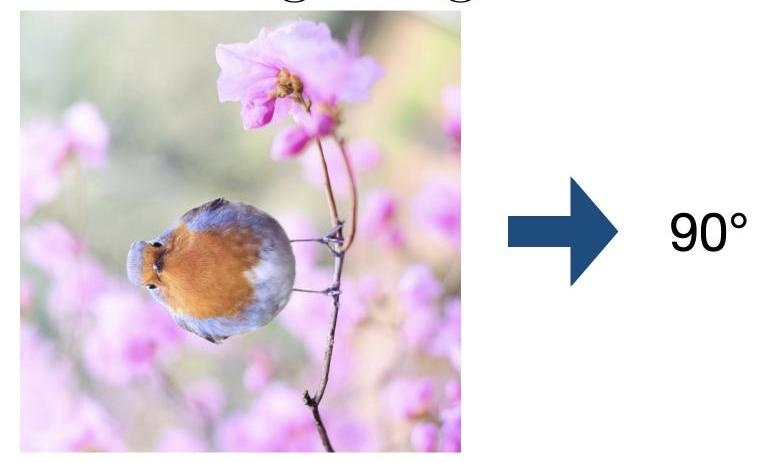
\includegraphics[max width=\textwidth]{2024_01_08_7c14f4867d7823fc5a52g-03}
\end{center}

Image Colorization:
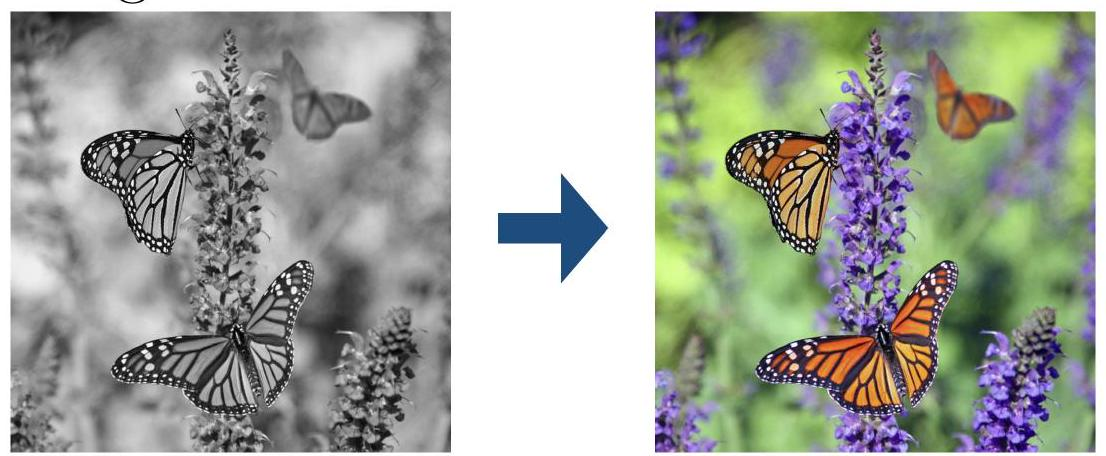
\includegraphics[max width=\textwidth, center]{2024_01_08_7c14f4867d7823fc5a52g-03(1)}

Predicting Relative Patch Placement:
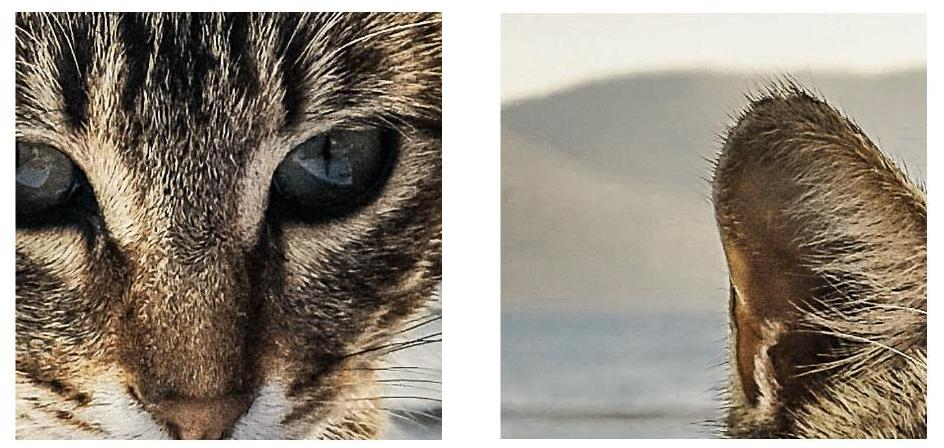
\includegraphics[max width=\textwidth, center]{2024_01_08_7c14f4867d7823fc5a52g-03(2)}

Second patch is above and left of the first

Upcoming:

\begin{itemize}
  \item Masked Language Modelling
  \item Next Token Prediction
\end{itemize}

\section*{Masked Language Modelling (MLM)}
Learn to predict masked (hidden) words for example: She [MASK] her coffee $\mapsto$ She drank her coffee

Forces the model to learn a comprehensive representation of the language that is very useful for many downstream tasks. Can train on huge corpora of text (books, Wikipedia, etc) without any labelling.

\section*{BERT}
Bidirectional Encoder Representations from Transformers is a well known family of language models based on the encoder-only transformer architecture and trained on masked language modelling.

Encoder: Sees the whole sequence at once, every token can generally attend to every other token (both previous and later ones, hence bidirectional). Generates a fixed sized output, typically one token per input.

\begin{center}
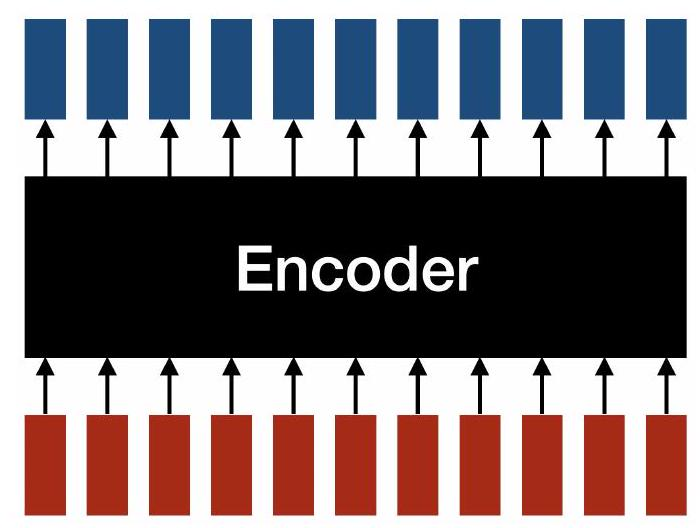
\includegraphics[max width=\textwidth]{2024_01_08_7c14f4867d7823fc5a52g-04}
\end{center}

Training Inputs: BERT is trained on input sequences consisting of two sentences and special tokens, for example:

[CLS] The cat is sleeping. [SEP] It's on the sofa. [SEP]

Where [CLS] is a special classification token and [SEP] is used to separate the two sentences. Around $15 \%$ of the standard tokens are selected to be replaced by [MASK]. Occasionally the selected tokens are replaced by a random word or not replaced to reduce distribution shift for downstream tasks that do not have [MASK]. Positional and segment encodings are added to the token embeddings.

\begin{center}
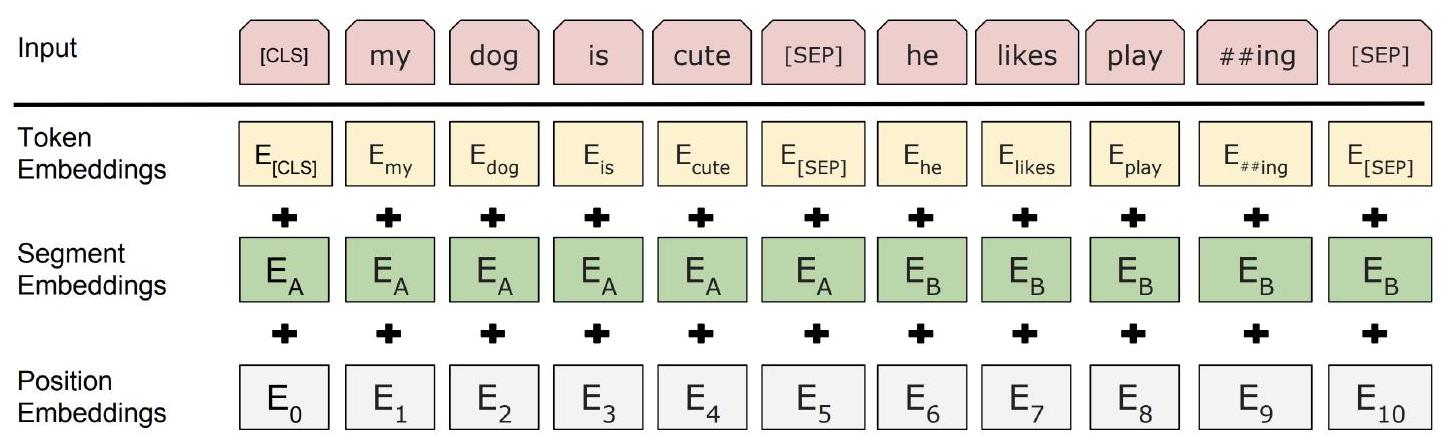
\includegraphics[max width=\textwidth]{2024_01_08_7c14f4867d7823fc5a52g-05}
\end{center}

Figure from the original BERT paper: \href{https://arxiv.org/abs/1810.04805}{https://arxiv.org/abs/1810.04805}

\section*{Training Objective:}
\begin{itemize}
  \item For each selected (replaced / masked) token: Predict the original token. Softmax cross-entropy loss over all possible tokens.
  \item For the [CLS] token: Predict whether the second sentence immediately follows the first sentence or not (binary classification).
\end{itemize}

Downstream tasks: The structure of the BERT training task allows fine-tuning for a variety of downstream tasks.

\begin{center}
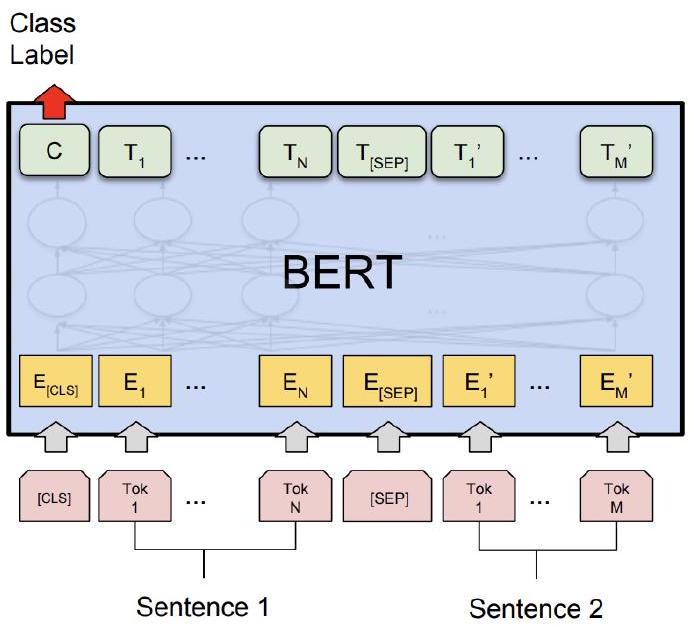
\includegraphics[max width=\textwidth]{2024_01_08_7c14f4867d7823fc5a52g-06(3)}
\end{center}

(a) Sentence Pair Classification Tasks: MNLI, QQP, QNLI, STS-B, MRPC, RTE, SWAG

\begin{center}
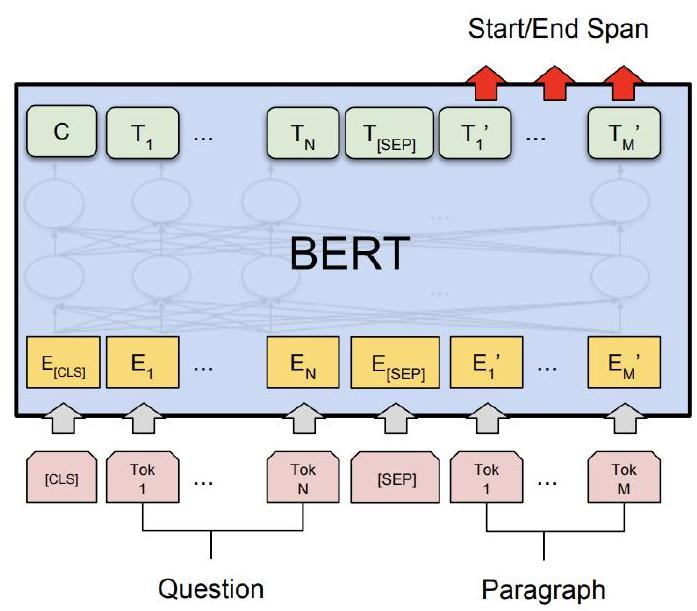
\includegraphics[max width=\textwidth]{2024_01_08_7c14f4867d7823fc5a52g-06(1)}
\end{center}

(c) Question Answering Tasks: SQUAD v1.1

\begin{center}
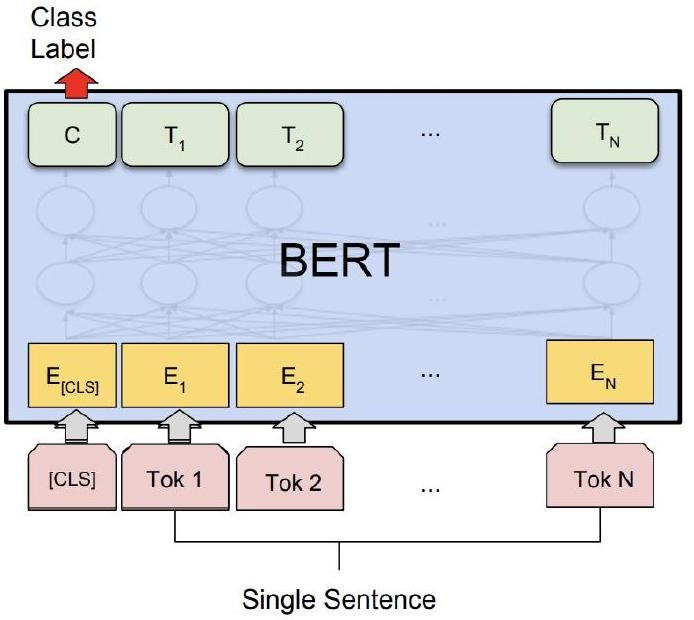
\includegraphics[max width=\textwidth]{2024_01_08_7c14f4867d7823fc5a52g-06}
\end{center}

(b) Single Sentence Classification Tasks: SST-2, CoLA

\begin{center}
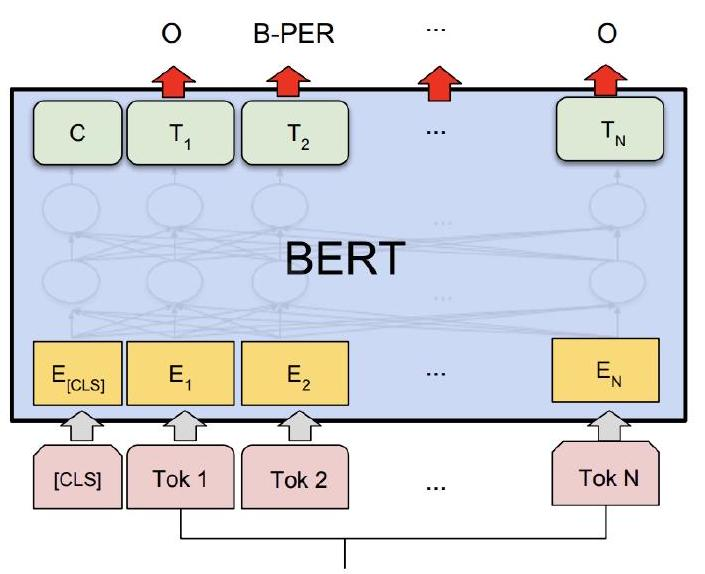
\includegraphics[max width=\textwidth]{2024_01_08_7c14f4867d7823fc5a52g-06(2)}
\end{center}

Single Sentence

(d) Single Sentence Tagging Tasks: CoNLL-2003 NER

Figure from the original BERT paper: \href{https://arxiv.org/abs/1810.04805}{https://arxiv.org/abs/1810.04805}

\begin{itemize}
  \item Classifying sentences or pairs (e.g. sentiment analysis): Use the [CLS] token.
  \item Word level classification (e.g. named entity recognition): Use the output for each token.
  \item Extracting a relevant passage (e.g. search): Use the individual outputs to define a span.
\end{itemize}

\section*{Next Token Prediction}
Predict the next token given previous tokens, e.g.: She drank her $\mapsto$ coffee

Similar to Masked Language Modelling but is causal, we can only see previous words, not later ones. This makes it better suited for generating arbitrary length responses.

\section*{GPT}
Generative Pre-trained Transformers are a family of language models based on the decoder-only transformer architecture and trained on next token prediction. Most generative Large Language Models (LLMs) like GPT-4 and LLAMA are members of this family. They can be fine tuned for a variety of purposes, famously as chatbots / assistants (ChatGPT, Bard).

Decoder: Each token can only attend to prior tokens (operates causally). Used autoregressively during inference, each generated output token is fed back into the model as an input to generate the following output token.

\begin{center}
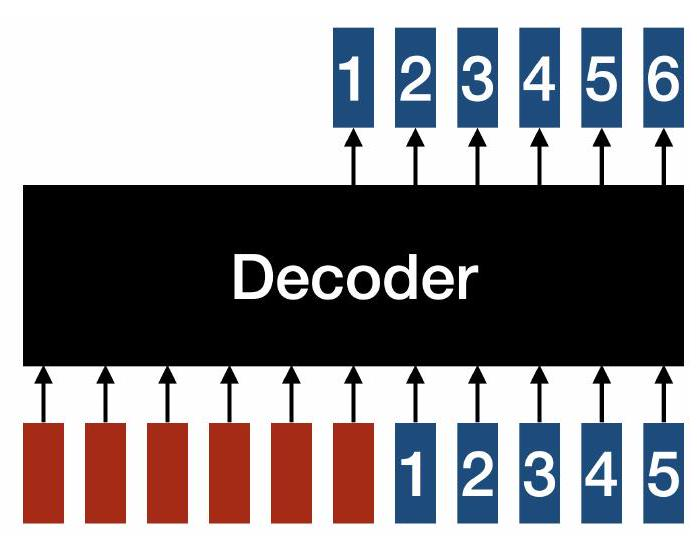
\includegraphics[max width=\textwidth]{2024_01_08_7c14f4867d7823fc5a52g-07}
\end{center}

Training Inputs: The training is simply done on token sequences with minimal changes e.g.:

[EOS] The cat is sleeping. It's on the sofa. [EOS]

Here the only special token used is [EOS] which signifies the end of text and is used to separate unrelated chunks of text (but this can vary between implementations).

Training Procedure: Standard training involves teacher forcing, where we don't use the model outputs as subsequent inputs (like in inference) but rather use the actual correct sequence. This allows training on all tokens in a sequence to happen in parallel rather than sequentially. We need to mask the attention to prevent tokens from attending to future tokens, preserving the causality needed for inference.

We obtain a loss for every token in the sequence corresponding to the prediction of the next token. This is a standard classification loss over the possible vocabulary (softmax cross-entropy). The total loss for a sequence is the mean loss over all tokens in the sequence.

Targets

Transformer With Masked Attention

Inputs

\begin{center}
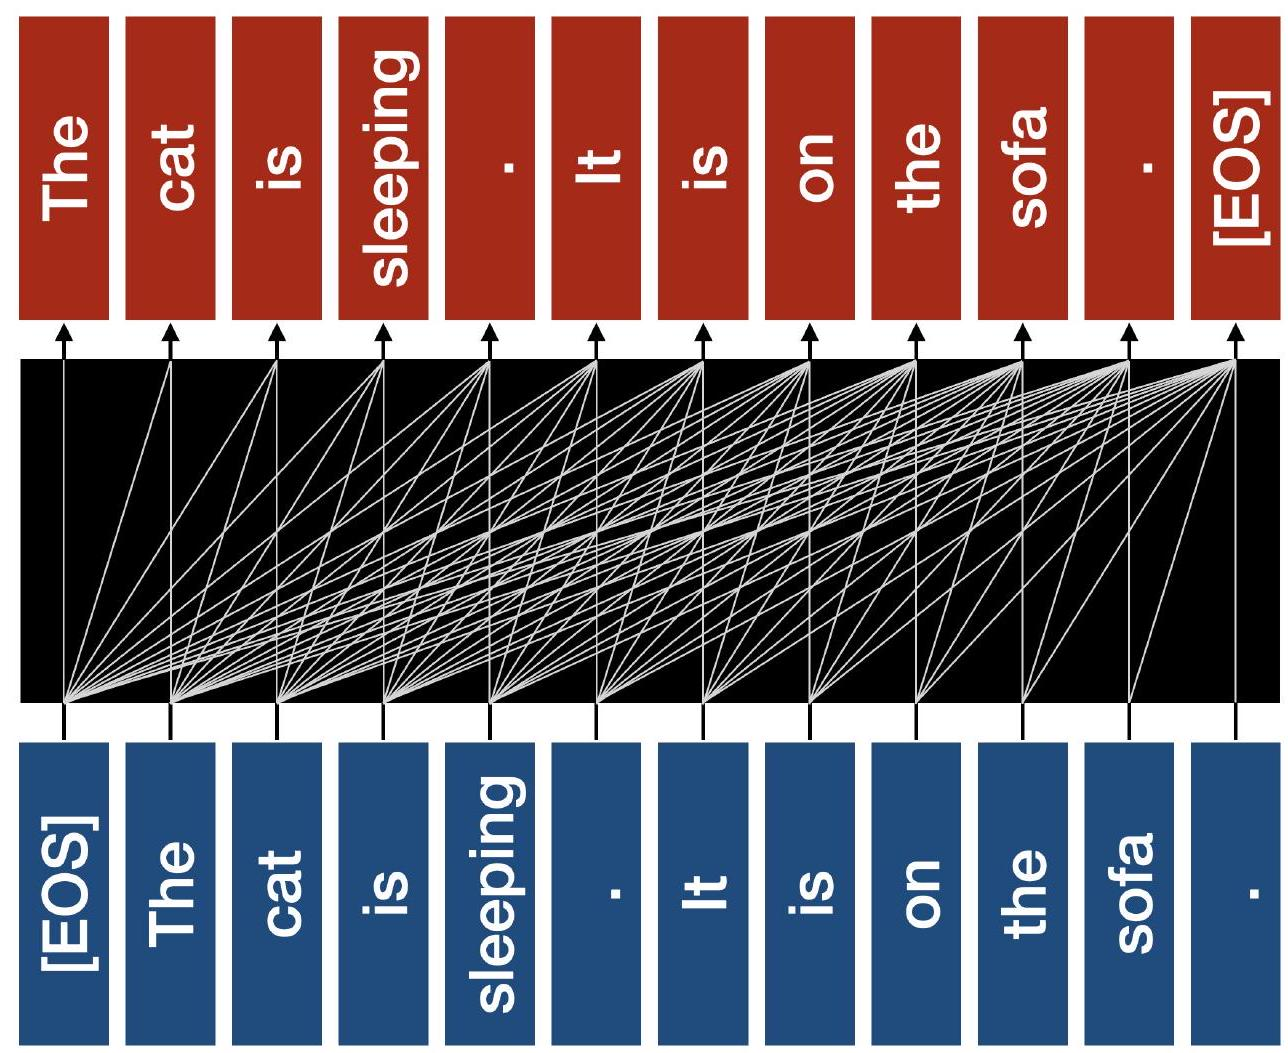
\includegraphics[max width=\textwidth]{2024_01_08_7c14f4867d7823fc5a52g-09}
\end{center}

Downstream Tasks: Decoders are very general sequenceto-sequence models and can be adapted to most natural language tasks. GPTs have been fine tuned for various applications. The base models are also often capable of performing various tasks without further tuning.

In-Context Learning: Large GPT models can sometimes complete new tasks with just a few examples of successful completion provided as inputs, without any model updates. The model uses patterns it has learned during its initial training to infer how to handle these new tasks. Example input:

Translate English to French: sea otter $=>$ loutre de mer cheese $=>$

which would hopefully result in fromage as an output.

The search for an effective input (prompt) to achieve desired output behavior is known as prompt engineering.

\section*{Joint Embedding Methods}
Learn an encoder invariant to certain transformations on the data, e.g., to rotation:
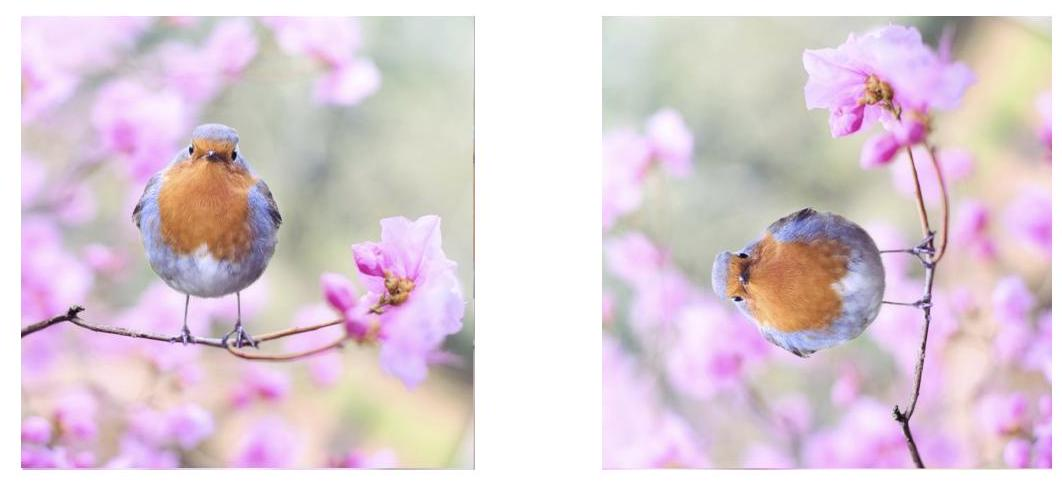
\includegraphics[max width=\textwidth, center]{2024_01_08_7c14f4867d7823fc5a52g-10}

Rather than learning a model $f$ :

$\mathbf{x}_{\text {in }} \mapsto \mathbf{x}_{\text {out }}$, learn $f: \mathcal{X} \rightarrow \mathbb{R}^{d}$ s.t.

$$
f\left(\mathbf{x}_{1}\right) \approx f\left(\mathbf{x}_{2}\right)
$$

where $g: \mathbf{x} \mapsto\left(\mathbf{x}_{1}, \mathbf{x}_{2}\right)$ is a transformation that creates two views from the same input datapoint $\mathbf{x} \in \mathcal{X}$.

$g$ is usually a random function that applies multiple data augmentations, each with certain probability.

Problem: constant $f$ is a trivial encoder that is invariant!

\begin{center}
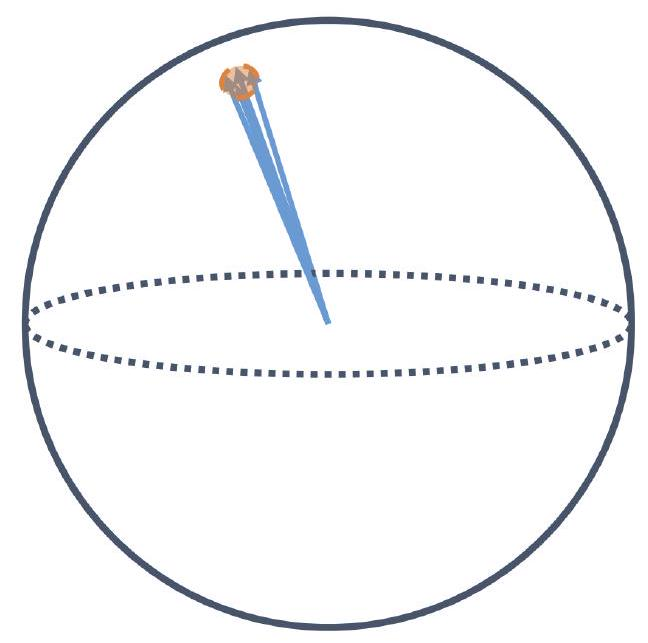
\includegraphics[max width=\textwidth]{2024_01_08_7c14f4867d7823fc5a52g-11}
\end{center}

Figure from \href{https://arxiv.org/abs/2110.09348}{https://arxiv.org/abs/2110.09348}

Solved by contrastive learning (next!) or non-contrastive methods with regularization, e.g.,

\begin{itemize}
  \item BYOL: use two encoders $f_{1}$, $f_{2}$ where $f_{2}$ is the exponential moving average of $f_{1}$ and force
\end{itemize}

$$
f_{1}\left(\mathbf{x}_{1}\right) \approx f_{2}\left(\mathbf{x}_{2}\right)
$$

\begin{itemize}
  \item VicReg: force non-zero variances to avoid collapse but minimize the covariance to reduce information overlap.
\end{itemize}

\section*{Contrastive learning}
Push away representations of unrelated views from different data points!
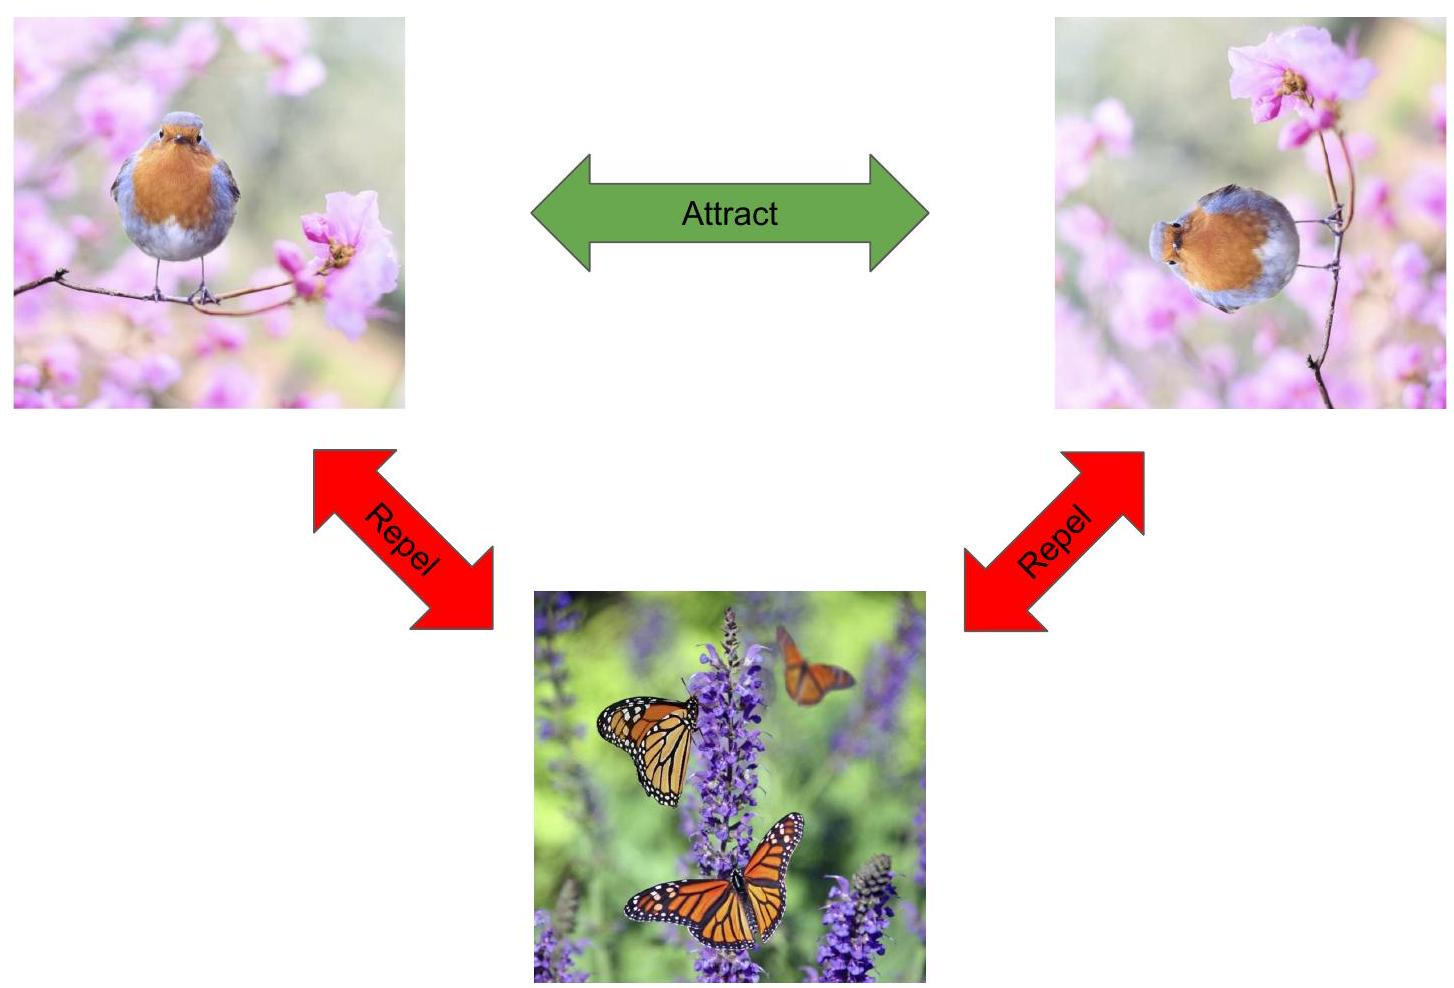
\includegraphics[max width=\textwidth, center]{2024_01_08_7c14f4867d7823fc5a52g-12}

Objective: given a positive pair $\mathbf{x}, \mathbf{x}^{+}$from the datapoint $\mathbf{x}$, and a negative view $\mathbf{x}^{-}$from a different datapoint $\mathbf{x}^{\prime} \neq \mathbf{x}$,

$\mathrm{s}\left(f(\mathbf{x}), f\left(\mathbf{x}^{+}\right)\right)>\mathrm{s}\left(f(\mathbf{x}), f\left(\mathbf{x}^{-}\right)\right)$,

where the s function quantifies the similarity of two embeddings.

\section*{SimCLR}
A contrastive learning framework with optimized choices.

\begin{enumerate}
  \item classification-like objective with $N$ negative samples:
\end{enumerate}

$$
L(\mathbf{x})=-\mathbb{E}\left[\log \frac{\exp \left(\mathrm{s}\left(f(\mathbf{x}), f\left(\mathbf{x}^{+}\right)\right)\right)}{\sum_{i=1}^{N} \exp \left(\mathrm{s}\left(f(\mathbf{x}), f\left(\mathbf{x}_{i}^{-}\right)\right)\right)}\right]
$$

\begin{itemize}
  \item maximize the score between $\mathbf{x}$ and $\mathbf{x}^{+}$,
  \item minimize the score between $\mathbf{x}$ and all $\mathbf{x}_{i}^{-}$.
\end{itemize}

\begin{enumerate}
  \setcounter{enumi}{1}
  \item use an additional projector to map the encoder output to the similarity (possibly lower-dimensional) space:
\end{enumerate}

$$
f(\mathbf{x})=\underbrace{f_{2}}_{\text {projector }} \circ \underbrace{f_{1}}_{\text {encoder }}(\mathbf{x})
$$

\begin{itemize}
  \item learn $f_{1}$ and $f_{2}$ jointly in an end-to-end fashion,
  \item use only $f_{1}$ for downstream tasks.
\end{itemize}

\begin{enumerate}
  \setcounter{enumi}{2}
  \item use cosine similarity with temperature scaling $\tau$ :
\end{enumerate}

$$
\mathrm{S}\left(\mathbf{e}_{1}, \mathbf{e}_{2}\right)=\frac{\left\langle\mathbf{e}_{1}, \mathbf{e}_{2}\right\rangle}{\left\|\mathbf{e}_{1}\right\|_{2}\left\|\mathbf{e}_{2}\right\|_{2}} / \tau
$$

\begin{enumerate}
  \setcounter{enumi}{3}
  \item generate views with data augmentation:
\end{enumerate}

\begin{center}
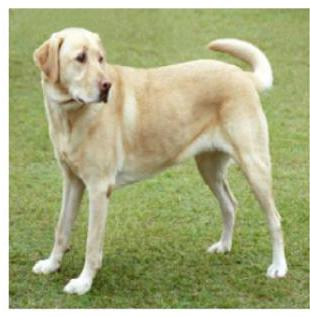
\includegraphics[max width=\textwidth]{2024_01_08_7c14f4867d7823fc5a52g-14(7)}
\end{center}

(a) Original

\begin{center}
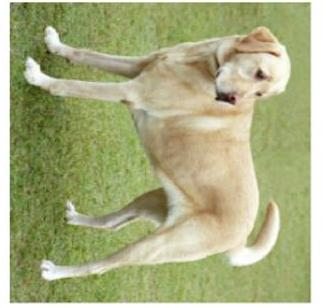
\includegraphics[max width=\textwidth]{2024_01_08_7c14f4867d7823fc5a52g-14(3)}
\end{center}

(f) Rotate $\left\{90^{\circ}, 180^{\circ}, 270^{\circ}\right\}$

\begin{center}
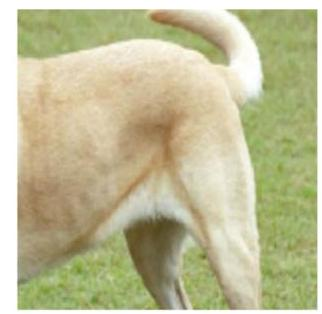
\includegraphics[max width=\textwidth]{2024_01_08_7c14f4867d7823fc5a52g-14(4)}
\end{center}

(b) Crop and resize

\begin{center}
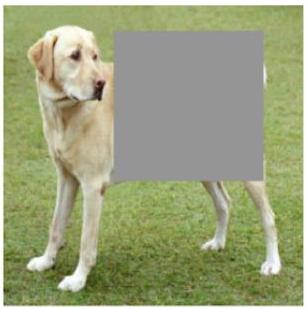
\includegraphics[max width=\textwidth]{2024_01_08_7c14f4867d7823fc5a52g-14(9)}
\end{center}

(g) Cutout

\begin{center}
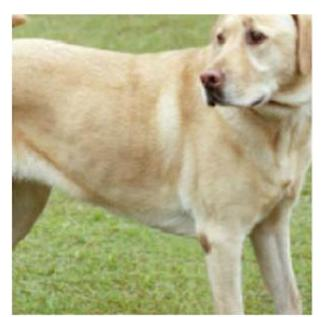
\includegraphics[max width=\textwidth]{2024_01_08_7c14f4867d7823fc5a52g-14(1)}
\end{center}

(c) Crop, resize (and flip)

\begin{center}
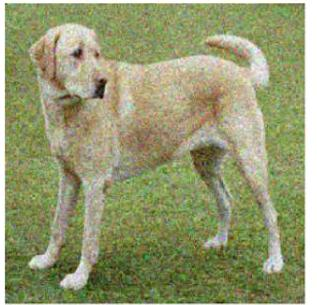
\includegraphics[max width=\textwidth]{2024_01_08_7c14f4867d7823fc5a52g-14(2)}
\end{center}

(h) Gaussian noise

\begin{center}
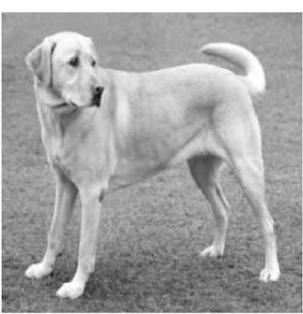
\includegraphics[max width=\textwidth]{2024_01_08_7c14f4867d7823fc5a52g-14(5)}
\end{center}

(d) Color distort. (drop)

\begin{center}
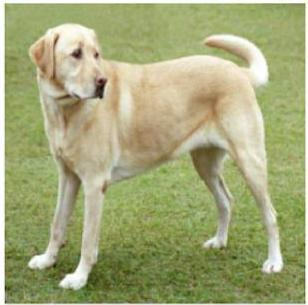
\includegraphics[max width=\textwidth]{2024_01_08_7c14f4867d7823fc5a52g-14(6)}
\end{center}

(i) Gaussian blur

\begin{center}
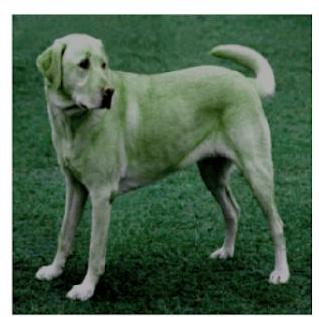
\includegraphics[max width=\textwidth]{2024_01_08_7c14f4867d7823fc5a52g-14}
\end{center}

(e) Color distort. (jitter)

\begin{center}
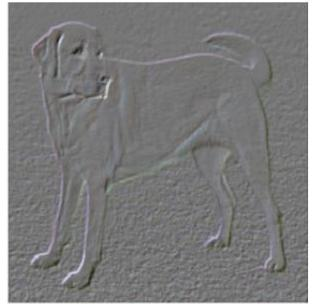
\includegraphics[max width=\textwidth]{2024_01_08_7c14f4867d7823fc5a52g-14(8)}
\end{center}

(j) Sobel filtering

Figure from the SimCLR paper: \href{https://arxiv.org/abs/2002}{https://arxiv.org/abs/2002}. 05709

\begin{itemize}
  \item stronger data augmentations than those used in supervised learning,
  \item random crop creates global to local $(B \rightarrow A)$ views or adjacent view $(D \rightarrow C)$ prediction tasks.
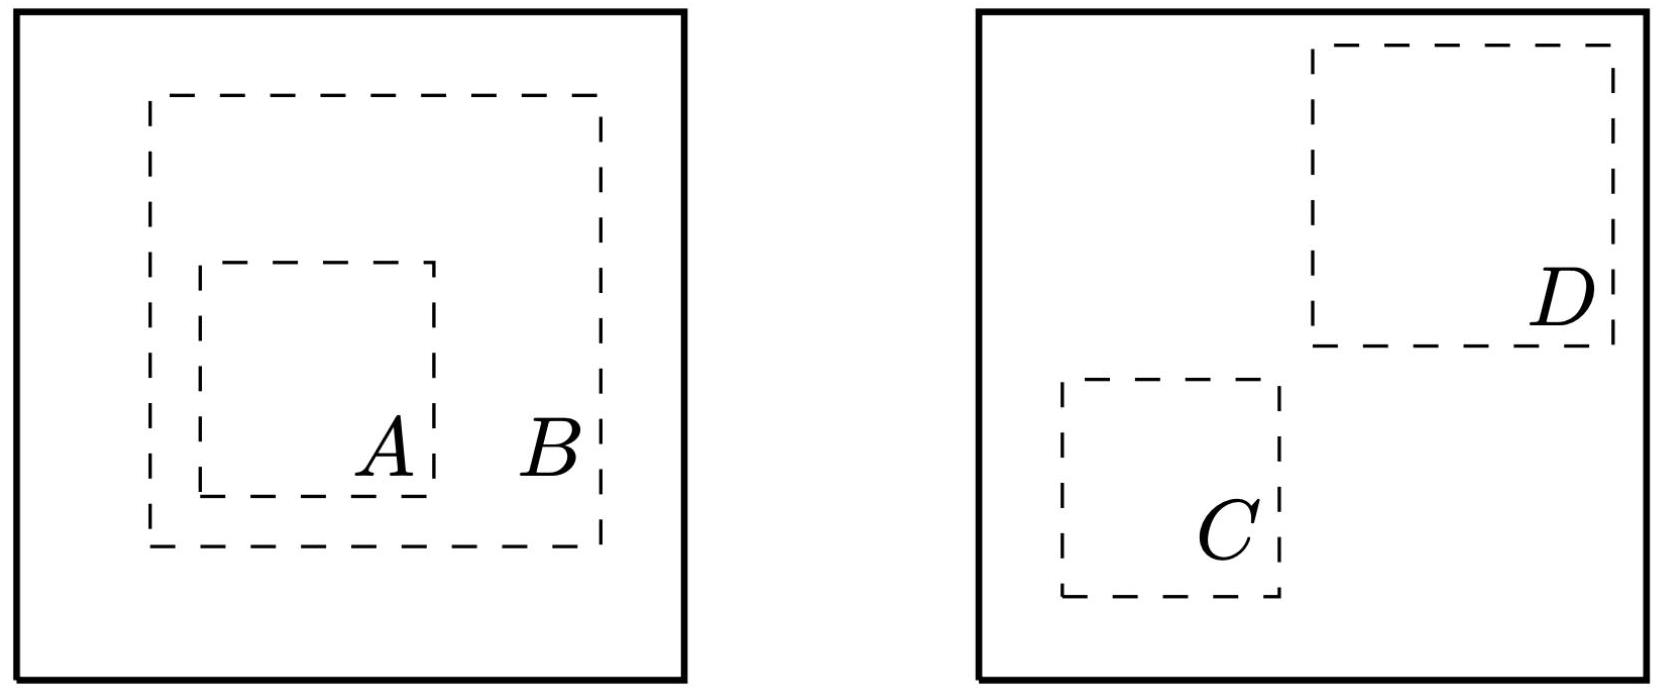
\includegraphics[max width=\textwidth, center]{2024_01_08_7c14f4867d7823fc5a52g-14(10)}
\end{itemize}

Figure from the SimCLR paper: \href{https://arxiv.org/abs/2002.05709}{https://arxiv.org/abs/2002.05709}

\section*{CLIP}
Use captioned images to learn a joint multimodal embedding space.

\begin{center}
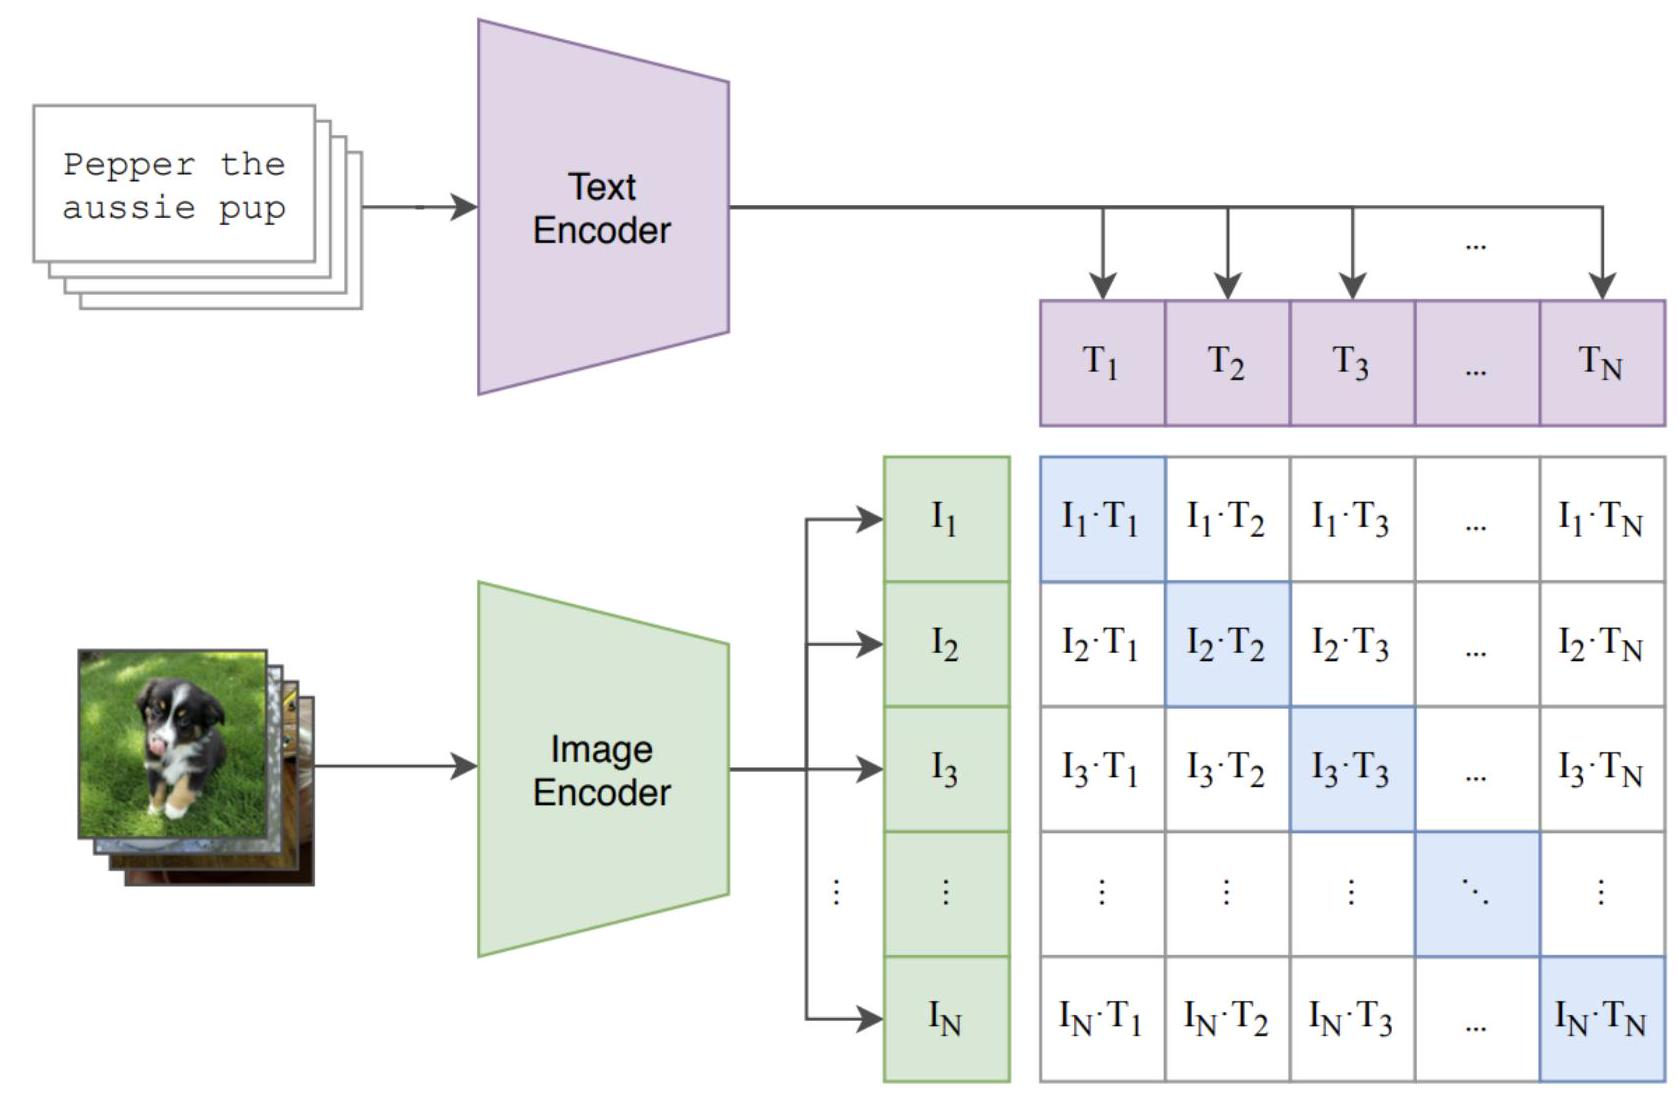
\includegraphics[max width=\textwidth]{2024_01_08_7c14f4867d7823fc5a52g-15}
\end{center}

Figure from the CLIP paper: \href{https://arxiv.org/abs/2103.00020}{https://arxiv.org/abs/2103.00020}

Objective: Maximize cosine similarity of caption and image embeddings while minimizing unrelated pairs.

Few-shot learning: learn to classify new classes with only a few labelled examples. CLIP is able to zero-shot classify with the following text input: "A photo of [class]".

\section*{Further Pointers}
\begin{enumerate}
  \item The Illustrated BERT:
\end{enumerate}

\href{https://jalammar.github.io/illustrated-bert/}{https://jalammar.github.io/illustrated-bert/}

\begin{enumerate}
  \setcounter{enumi}{1}
  \item The Illustrated GPT:
\end{enumerate}

\href{https://jalammar.github.io/illustrated-gpt2/}{https://jalammar.github.io/illustrated-gpt2/}


\end{document}